\chapter{Assessment of Renal $T_2$ Mapping Methods}
\label{chap:t2_mapping}
\newpage
\begin{abstract}
	Renal \ttwo mapping shows promising early results for the evaluation of multiple pathologies, however, of the few studies there is very little consistency due to the differing methodologies being employed across research groups. Here the four most common \ttwo mapping sequences for use in the kidneys, basic \ac{SE}-\ac{EPI}, \ac{ME-TSE}, \ac{GraSE} and \ac{CPMG} \ttwo preparation methods, are evaluated.
	
	Each of the four sequences was used to image a phantom designed by the \ac{NIST} with an array of spheres of known \ttwo to evaluate quantitative accuracy across the range of \ttwo values reported in the kidneys. The sensitivity of each sequence to flow was evaluated using a \ac{QASPER} phantom over a range of flow rates. Additionally, the image quality of each sequence was assessed by estimating the point spread function. All sequences were then used to acquire \ttwo maps of five healthy volunteers. 
	
	In the \ac{NIST} phantom, the basic spin echo sequence delivered the most accurate quantitative results over the range of \ttwo reported in the kidneys (40 sm - 200 ms), however its sensitivity to flow and wide point spread function limit its use in-vivo. Instead, a gradient spin echo sequence is recommended, with a mean relative error of 15 $\pm$ 4~\% over the range of \ttwo reported within the kidneys (40 ms – 200 ms), superior readability due to its smaller point spread function and insensitivity to flow.
	
	\textit{This work was presented as an oral presentation at the \ac{ISMRM} 28th Annual Meeting (2020) \cite{daniel_comparison_2020}.}
	
%	\lipsum[1]
\end{abstract}
\newpage
\acresetall

\section{Introduction}
\label{sec:t2_intro}

\subsection{Motivation}
Quantitative \ac{MRI} is the process of taking measurements where the voxel values have numerical significance rather than simply representing signal intensity in arbitrary units \cite{tofts_quantitative_2003}. These numerically significant values can take the form of macroscale properties such as rate of oxygen consumption and blood vessel flow rates or microscale properties such as tissue \tone, \ttwo, diffusion and susceptibility. When interpreted, these values may provide useful biomarkers for improved diagnosis and treatment of patients.

The kidneys are structurally and functionally complex organs and as such lend themselves to the wide variety of \ac{MRI} protocols designed to probe different aspects of the tissue and processes carried out within, termed multiparametric \ac{MRI}. While high resolution images of the kidneys morphology and basic measures such as \ac{TKV} can be very useful in diagnosing and monitoring disease progression \cite{buchanan_quantitative_2019, chapman_kidney_2012, gong_relationship_2012}, these do not fully leverage the quantitative nature of \ac{MRI}. Measurements of \tone have been shown to correlate well with fibrosis in the myocardium \cite{bull_human_2013, ferreira_t1_2013}, liver \cite{hoad_study_2015, luetkens_quantification_2018} and kidneys \cite{friedli_new_2016} and an increase in \tone has been associated with \ac{CKD} \cite{gillis_non-contrast_2016, cox_multiparametric_2017, buchanan_quantitative_2019}. \ac{ASL} techniques can be used to quantify renal perfusion in physiological units (m$\ell$/100g/min) and have been shown to correlate with allograft function post renal transplant in addition to cold ischemia time and the recipients \ac{eGFR} \cite{hueper_functional_2015, artz_arterial_2011, ren_evaluation_2016, niles_longitudinal_2016}. \ac{ASL} has been used to demonstrate a decrease in perfusion in \ac{CKD} subjects \cite{gillis_non-contrast_2016, rossi_histogram_2012, tan_renal_2014}. These techniques have proved useful when used in isolation however they can be combined and used in the same scanning session to greater effect within a multiparametric protocol \cite{buchanan_quantitative_2019, cox_multiparametric_2017, eckerbom_multiparametric_2019, schley_multiparametric_2018, hueper_kidney_2016}.

\ttwo mapping has found wide use in cardiac \ac{MRI} for the assessment of myocardial oedema \cite{gouya_rapidly_2008, giri_t2_2009, nasenstein_cardiac_2014} and iron overload \cite{guo_myocardial_2009, krittayaphong_detection_2017}. \ttwo mapping has also effectively been used in the brain to study multiple sclerosis \cite{neema_t1-_2007}, epilepsy \cite{rugg-gunn_whole-brain_2005}, dementia \cite{knight_quantitative_2016} and Parkinson’s disease \cite{vymazal_t1_1999}. Despite these developments elsewhere in the body, \ttwo mapping has had limited uptake in the renal community.

Renal \ttwo mapping has seen most research focusing on repeatability measures \cite{de_bazelaire_mr_2004, zhang_reproducibility_2011, li_measuring_2015, de_boer_multiparametric_2020} with clinical uses in the field of assessment of allograft function in mice \cite{hueper_kidney_2016} and humans \cite{mathys_t2_2011, adams_multiparametric_2020}, and has shown potential for early diagnosis of \ac{ADPKD} \cite{franke_magnetic_2017} and assessment of clear cell renal cell carcinoma \cite{adams_use_2019}.

In the existing literature, there is a substantial variation in quoted \ttwo values within the kidneys of healthy volunteers, Table \ref{tab:t2_lit_values}, this is thought to be, in part, due to the differences in \ttwo mapping methodologies. There are currently four main \ttwo mapping methods that have been published in the kidneys: basic \ac{SE}-\ac{EPI}, \ac{ME-TSE}, \ac{GraSE} and \ac{CPMG} \ttwo preparation. 

\begin{table}[H]
	\centering
	\begin{adjustbox}{width=1.0\textwidth, center}
	\begin{tabularx}{1.32\textwidth}{XXXXXX}
		\multicolumn{1}{l|}{Author}                                         & \multicolumn{1}{l|}{Year} & \multicolumn{1}{l|}{Sample Size} & \multicolumn{1}{l|}{Sequence}        & \multicolumn{1}{l|}{Cortex \ttwo (ms)} & Medulla \ttwo (ms) \\ \hline
		\multicolumn{6}{c}{{\textbf{3T}}}                                                                                                                                                                                                                  \\ \hline
		\multicolumn{1}{l|}{de Bazelaire \textit{et al} \cite{de_bazelaire_mr_2004}} & \multicolumn{1}{l|}{2004} & \multicolumn{1}{l|}{6}           & \multicolumn{1}{l|}{SE \ttwo prep}   & \multicolumn{1}{l|}{76 $\pm$ 7}        & 81 $\pm$ 8         \\ \hline
		\multicolumn{1}{l|}{Li \textit{et al} \cite{li_measuring_2015}}              & \multicolumn{1}{l|}{2015} & \multicolumn{1}{l|}{5}           & \multicolumn{1}{l|}{CPMG \ttwo prep} & \multicolumn{1}{l|}{121 $\pm$ 5}       & 138 $\pm$ 7        \\ \hline
		\multicolumn{1}{l|}{Franke \textit{et al} \cite{franke_magnetic_2017}}       & \multicolumn{1}{l|}{2017} & \multicolumn{1}{l|}{3}           & \multicolumn{1}{l|}{GraSE}           & \multicolumn{1}{l|}{132 $\pm$ 6}       &                    \\ \hline
		\multicolumn{1}{l|}{Adams \textit{et al} \cite{adams_multiparametric_2020}}  & \multicolumn{1}{l|}{2020} & \multicolumn{1}{l|}{16}          & \multicolumn{1}{l|}{GE \ttwo prep}   & \multicolumn{1}{l|}{78 $\pm$ 4}        & 59 $\pm$ 2         \\ \hline
		\multicolumn{6}{c}{{ \textbf{1.5T}}}                                                                                                                                                                                                                \\ \hline
		\multicolumn{1}{l|}{de Bazelaire \textit{et al} \cite{de_bazelaire_mr_2004}} & \multicolumn{1}{l|}{2004} & \multicolumn{1}{l|}{4}           & \multicolumn{1}{l|}{SE \ttwo prep}   & \multicolumn{1}{l|}{87 $\pm$ 4}        & 85 $\pm$ 11        \\ \hline
		\multicolumn{1}{l|}{Zhang \textit{et al} \cite{zhang_reproducibility_2011}}  & \multicolumn{1}{l|}{2011} & \multicolumn{1}{l|}{4}           & \multicolumn{1}{l|}{2D ME-TSE}       & \multicolumn{1}{l|}{112 $\pm$ 8}       & 137$\pm$ 13        \\ \hline
		\multicolumn{1}{l|}{Mathys \textit{et al} \cite{mathys_t2_2011}}             & \multicolumn{1}{l|}{2011} & \multicolumn{1}{l|}{6}           & \multicolumn{1}{l|}{ME-SE}           & \multicolumn{1}{l|}{125$\pm$ 7}        &                    \\ \hline
		\multicolumn{1}{l|}{Siedek \textit{et al} \cite{siedek_magnetic_2020}}       & \multicolumn{1}{l|}{2020} & \multicolumn{1}{l|}{10}          & \multicolumn{1}{l|}{GraSE}           & \multicolumn{1}{l|}{130 $\pm$ 6}       &                   
	\end{tabularx}
	\end{adjustbox}
	\caption{Studies documenting renal \ttwo in healthy volunteers at 3T and 1.5T. This is an updated table from Wolf \textit{et al} \cite{wolf_magnetic_2018}.}
	\label{tab:t2_lit_values}
\end{table}

\newpage
Here each of these four methods are compared in the context of renal \ttwo mapping to ascertain which is most suitable. This is achieved by evaluating each methods quantitative accuracy, image quality, sensitivity to flow in phantoms and suitability for use in-vivo in final evaluation across five healthy subjects.

\subsection{Common Sources of Error in \ttwo Mapping Sequences}
The basic principles of \ttwo mapping are outlined in Section \ref{subsec:theory_t2}, these principles can be achieved using multiple methods, described in Section \ref{subsec:t2_acquisition_schemes}, however many of these methods have common sources of error leading to inaccuracies in measured \ttwo. 

\subsubsection{Diffusion}
\ttwo mapping sequences negate $T_2'$ effects cause by static $B_0$ inhomogeneities by refocusing this mechanism of signal attenuation. This is possible because, if spins are in an area of slightly higher magnetic field than $B_0$ they will de-phase quicker than spins in an area at $B_0$. Upon the application of a 180$\degree$ \ac{RF} pulse the spins being to re-phase, with those in areas of slightly higher magnetic field precessing quicker and ultimately causing an echo with the effects of static field inhomogeneities negated. This technique relies upon the environment each spin is in remaining constant before and after the 180$\degree$ pulse to achieve purely \ttwo weighted echoes. The movement of molecules via diffusion violates this requirement as spins can move into an area of slightly different magnetic field and thus precess are different rates before and after the 180$\degree$ refocusing pulse, causing an attenuation in transverse magnetisation above that of \ttwo \cite{carr_effects_1954}.

\subsubsection{Outflow}

Multi-slice imaging uses slice selective \ac{RF} pulses to image one slice while the longitudinal magnetisation of other slices is returning to equilibrium. This allows excitation to occur at a rate quicker than five times \tone as slices can be acquired without affecting the preceding or next slice to be acquired. The use of slice selective \ac{RF} pulses leads to potential outflow artefacts. These occur when the spin in an imaging plane flows out of the plane and is replaced by another spin and as such the full pulse sequence isn't delivered to the same spin. As the slice thickness of these schemes is typically in the order of 5 mm, a significant proportion of the excited spins within a voxel can be replaced in the tens to hundreds of milliseconds between excitation and acquisition. This results in artificially reduced signal with the effect becoming more prominent as echo time increases thus leading to underestimations of \ttwo.

\subsubsection{RF Pulse Imperfections}

Some \ttwo mapping schemes involve long trains of successive  \ac{RF} pulses. These pulses need to be very accurate to ensure that the spin ensemble is evolving as expected however this is not possible for multiple reasons, including but not limited to, pulse profile imperfections \cite{majumdar_errors_1986}, $B_0$ inhomogeneities \cite{majumdar_errors_1986-1} and slice profile imperfections \cite{crawley_errors_1987}.

Upon the application of an imperfect 180$\degree$ refocusing pulse, an ensemble of spins can be decomposed into three components, a transverse component that rephrases i.e. the desired behaviour, a transverse component that continues to de-phase and a longitudinal component with the proportion of the initial magnetisation in each component being dependent on the accuracy of the refocusing pulse. This splitting of magnetisation results in a reduced intensity echo. 

As subsequent refocusing pulses are applied, each of the split components can further split into three components resulting in large numbers of potential phase evolutions. Some of the possible phase evolutions will not form an echo between every refocusing pulse and as such the point at which the additional signal due to alternative paths will contribute to an echo in the train is difficult to predict. 

The many potential paths a spin ensemble can take can be represented using \acp{EPG}, an example of which is shown for four refocusing pulses in Figure \ref{fig:t2_epg}. If all refocusing pulses were perfect, the magnetisation would remain on the red path forming an echo every time the path crosses the $x$-axis (blue circles). If imperfect refocusing pulses are applied, the magnetisation splits at the first refocusing pulse where a component follows the initial red path, another component continues to de-phase in the transverse plane (green path) and another component is shifted to the longitudinal plane (blue path) and undergoes \tone relaxation. The example alternative path shown in blue does not contribute to the first echo but does contribute to the intensity of the second echo, the green path contributes to the intensity of the third echo.

\begin{figure}[H]
	\centering
	\includegraphics[width=0.6\textwidth]{T2_Mapping/EPG/EPG-01.eps}
	\caption{The \ac{EPG} produced from four successive imperfect refocussing pulses. The simple path shown in red produces an echo every time it crosses the $x$-axis while the more complex paths shown in blue and green only contribute to the intensity of the second and third echoes respectively.}
	\label{fig:t2_epg}	
\end{figure}

\subsection{\ttwo Acquisition Schemes}
\label{subsec:t2_acquisition_schemes}
Below the four methods to be compared in the context of renal imaging are outlined.

\subsubsection{Spin Echo-Echo Planar Imaging}
The \acf{SE}-\acf{EPI} technique is the simplest of the four methods, and so achievable on any \ac{MRI} scanner, and consists of a 90$\degree$ excitation pulse, followed by a 180$\degree$ \ac{RF} pulse \ac{TE}/2 ms later, leading to an echo at \ac{TE}. The 180$\degree$ pulse corrects for components of the signal lost due to static field inhomogeneities, $T_2'$ effects, however does not correct for \ttwo effects. By repeating the sequence multiple times with a different \ac{TE}, the \ttwo decay can be sampled. An \ac{EPI} readout is used to sample the signal during the echo. The relatively long \ac{TR} of this scheme means multiple slices can be sampled within a single \ac{TR}. In this case, the acquisition of each echo time is divided into two packages with odd numbered slices being sampled in the first \ac{TR} and even numbered slices being sampled in the second \ac{TR} to avoid contamination across slices due to the width of the slice selected by the 180$\degree$ refocussing pulse. An overview of the sequence is shown in Figure \ref{fig:t2_se-epi_seq}.

\begin{figure}[H]
	\centering
	\includegraphics[width=0.7\textwidth]{T2_Mapping/Pulse_Diagrams/T2_SE_EPI.eps}
	\caption{A pulse sequence diagram of the \acsu{SE}-\ac{EPI} scheme. Data is collected by repeating the acquisition across repetitions with different echo times.}
	\label{fig:t2_se-epi_seq}	
\end{figure}

\newpage
\subsubsection{Multi-Echo Turbo Spin Echo}
The \acf{ME-TSE} sequence comprises a series of 180$\degree$ pulses with an echo forming between each. Unlike in Section \ref{subsubsec:theory_tse}, where every echo was collecting a different line of $k$-space, here the same line of $k$-space is collected at a different \ac{TE}. This allows the whole \ttwo decay to be sampled in a single echo train. Different echo times are sampled by varying the number and spacing of the 180$\degree$ pulses, the number of echoes is limited by the \ac{TSE} factor. If a \ac{TSE} factor of twice the number of echoes is used, two lines of $k$-space can be collected per excitation, however this results in much longer echo trains and as such reduced \ac{SNR} and quantitative accuracy. By using a multi-slice acquisition, many slices can be acquired per \ac{TR}, meaning that for the small number of slices usually imaged in the body and if \ac{TSE} factor is equal to the number of echoes, the number of \acp{TR} required is simply the number of lines of $k$-space sampled. A schematic of the \ac{PSD} can be seen in Figure \ref{fig:t2_me-tse_seq}.

\begin{figure}[H]
	\centering
	\includegraphics[width=0.7\textwidth]{T2_Mapping/Pulse_Diagrams/T2_ME_TSE.eps}
	\caption{A pulse sequence diagram of the \ac{ME-TSE} scheme for a given \ac{TR}. If multiple lines of $k$-space are sampled per excitation, phase encode `blips' will not be consistent over the echo train.}
	\label{fig:t2_me-tse_seq}	
\end{figure}

\newpage
\subsubsection{Gradient Spin Echo}

To achieve further acceleration over the \acf{ME-TSE} sequence, a \ac{GraSE} sequence can be used. Here two gradient echoes are collected for every spin echo; the spin echo and gradient echo are used for the acquisition of the centre and periphery of $k$-space respectively. \ac{GraSE} sequences tend to use shorted \ac{RF} pulses and as such this enables a decrease in the echo spacing of the \ac{GraSE} sequence compared to the \ac{ME-TSE} sequence. The first echo of the train has an artificially high signal, however the short echo spacing of this technique means a startup echo can be sacrificed i.e. in this work the first echo is sampled at 11.2 ms (twice the echo spacing) rather than 5.6 ms. This leads to a more accurate fit, while also retaining accuracy when measuring short $T_2$ signals that will quickly decay. The \ac{PSD} for the \ac{GraSE} acquisition is shown in Figure \ref{fig:t2_grase_seq}.

\begin{figure}[H]
	\centering
	\includegraphics[width=0.7\textwidth]{T2_Mapping/Pulse_Diagrams/T2_GraSE.eps}
	\caption{A pulse sequence diagram of the \ac{GraSE} scheme.}
	\label{fig:t2_grase_seq}	
\end{figure}

\newpage
\subsubsection{CPMG $T_2$ Preparation}

As in the other sequences, the \ac{CPMG} sequence begins with a 90$\degree$ excitation pulse to transfer the magnetisation into the transverse plane. Carr and Purcell showed that a series of 180$\degree$ pulses of alternating phase could be used to reduce the effects of molecular diffusion \cite{carr_effects_1954}. This technique relies on very accurate 180$\degree$ pulses as small imperfections could result in large cumulative errors over the length of the pulse train. Later Meiboom and Gill showed that by delivering the 180$\degree$ pulses 90$\degree$ out of phase to the initial excitation pulse e.g. excite about $x'$ and refocus about $y'$, the undesirable effects of imperfect 180$\degree$ pulses and $B_1$ inhomogeneity could be greatly reduced \cite{meiboom_modified_1958}. The resulting sequence, known as a \acf{CPMG} sequence, can be used to generate robust measurements of \ttwo; by varying the number and temporal spacing, $\tau_{\textup{CPMG}}$, of the 180$\degree$ pulses the degree of \ttwo weighting can me modulated to achieve different \ac{eTE}. This sequence is not widely available and as such has been coded for the Philips platform specifically for this work. Here an \ac{EPI} readout scheme is then used to sample the signal. An overview of this sequence is shown in Figure \ref{fig:t2_cpmg_t2prep_seq}.

\begin{figure}[H]
	\centering
	\includegraphics[width=0.7\textwidth]{T2_Mapping/Pulse_Diagrams/T2_T2_Prep.eps}
	\caption{A pulse sequence diagram of the \ac{CPMG} $T_2$ preparation scheme. This example is shown for four \ac{CPMG} refocusing pulses, to achieve a longer \ac{eTE} the number of refocusing pulses is increased.}
	\label{fig:t2_cpmg_t2prep_seq}	
\end{figure}

\subsubsection{Multi-Echo Spin-Echo}
In addition to the four techniques above which can be applied in the required time frame for in-vivo measurements, a Multi-Echo Spin-Echo scheme was used to evaluate the quantitative accuracy of the phantom. This scheme is recommended by \ac{NIST} for use with their phantom to validate scanner hardware. It is however, impractical to implement in-vivo due to its very long acquisition time (16 minutes for a single slice). The sequence is similar to the \ac{ME-TSE} sequence, however, no fast imaging techniques are employed to achieve maximum \ac{SNR}, additionally, this sequence can only ever collect one line of $k$-space per excitation. A \ac{PSD} for this scheme is shown in Figure \ref{fig:t2_me-se_seq}.

\begin{figure}[H]
	\centering
	\includegraphics[width=0.7\textwidth]{T2_Mapping/Pulse_Diagrams/T2_ME_SE.eps}
%	\missingfigure{ME-SE Scheme (ME-TSE PSD with all but the first PE blip removed and one extra echo).}
	\caption{A pulse sequence diagram of the Multi-Echo Spin-Echo scheme.}
	\label{fig:t2_me-se_seq}	
\end{figure}

\newpage

\section{Methods}
\label{sec:t2_methods}

\subsection{Phantom Data Acquisition}

All data was acquired on a 3T Philips Ingenia system (Philips Medical Systems, Best, The Netherlands). The 14 element \ttwo array of a QalibreMD System Standard Model 130 contains spheres doped with varying concentrations of \ce{MnCl_2} to modulate \ttwo between 5 ms and 650 ms, Figure \ref{fig:t2_phantom_schematic}. This array was used to compare the accuracy of \ttwo measurements to a known ground truth. Additionally, a square grid etched into the plastic of the phantom was used to assess the degree of image blurring. 

%\begin{figure}[H]
%	\centering
%	\includegraphics[width=0.5\textwidth]{T2_Mapping/Phantom_Example/T2_Spheres.eps}
%	\caption{A schematic of the $T_2$ spheres in the QalibreMD phantom.}
%	\label{fig:t2_phantom_schematic}	
%\end{figure}
%\begin{figure}[H]
%	\centering
%	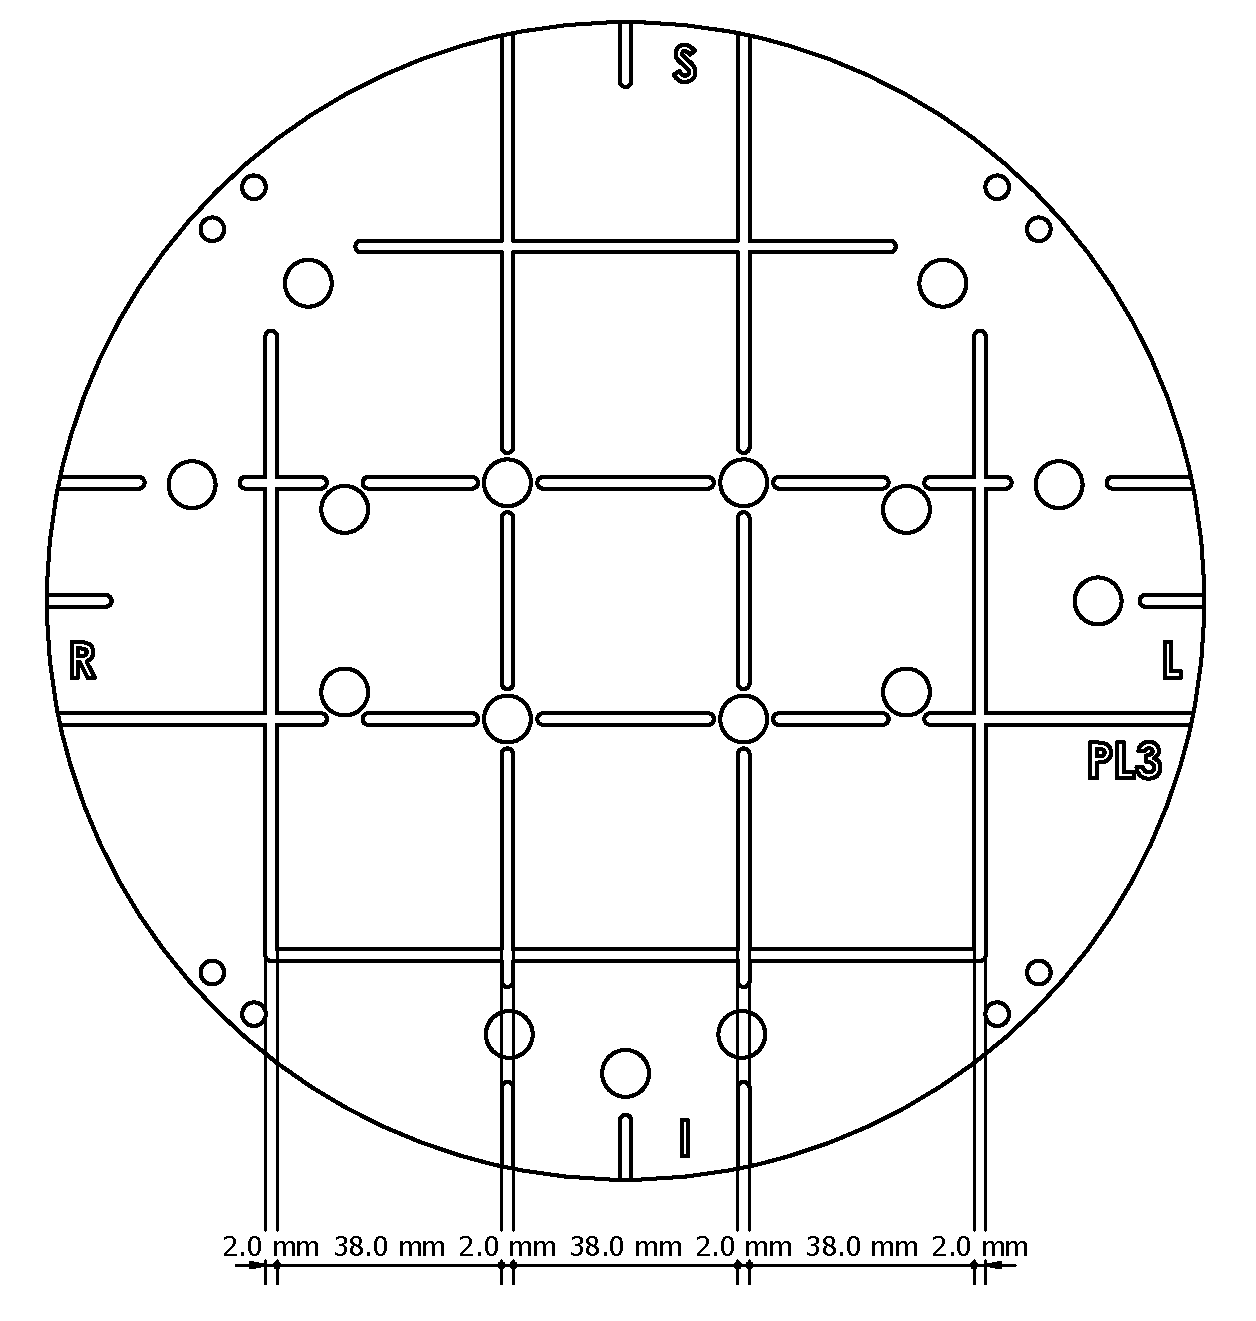
\includegraphics[width=0.6\textwidth]{T2_Mapping/2D_Blur/Plate_3_Grid_crop.pdf}
%	\caption{A scale drawing of plate three of the QalibreMD system phantom. The grid etched into this plate was used to assess the blurring of each \ttwo mapping sequence.}
%	\label{fig:t2_blur_grid}	
%\end{figure}
\begin{figure}[H]
\centering
\begin{subfigure}[c]{0.47\textwidth}
	\centering
	\includegraphics[width=1\textwidth]{T2_Mapping/Phantom_Example/T2_Spheres.eps}
	\caption{}
	\label{fig:t2_phantom_schematic}
\end{subfigure}
\hfill
\begin{subfigure}[c]{0.47\textwidth}
	\centering
	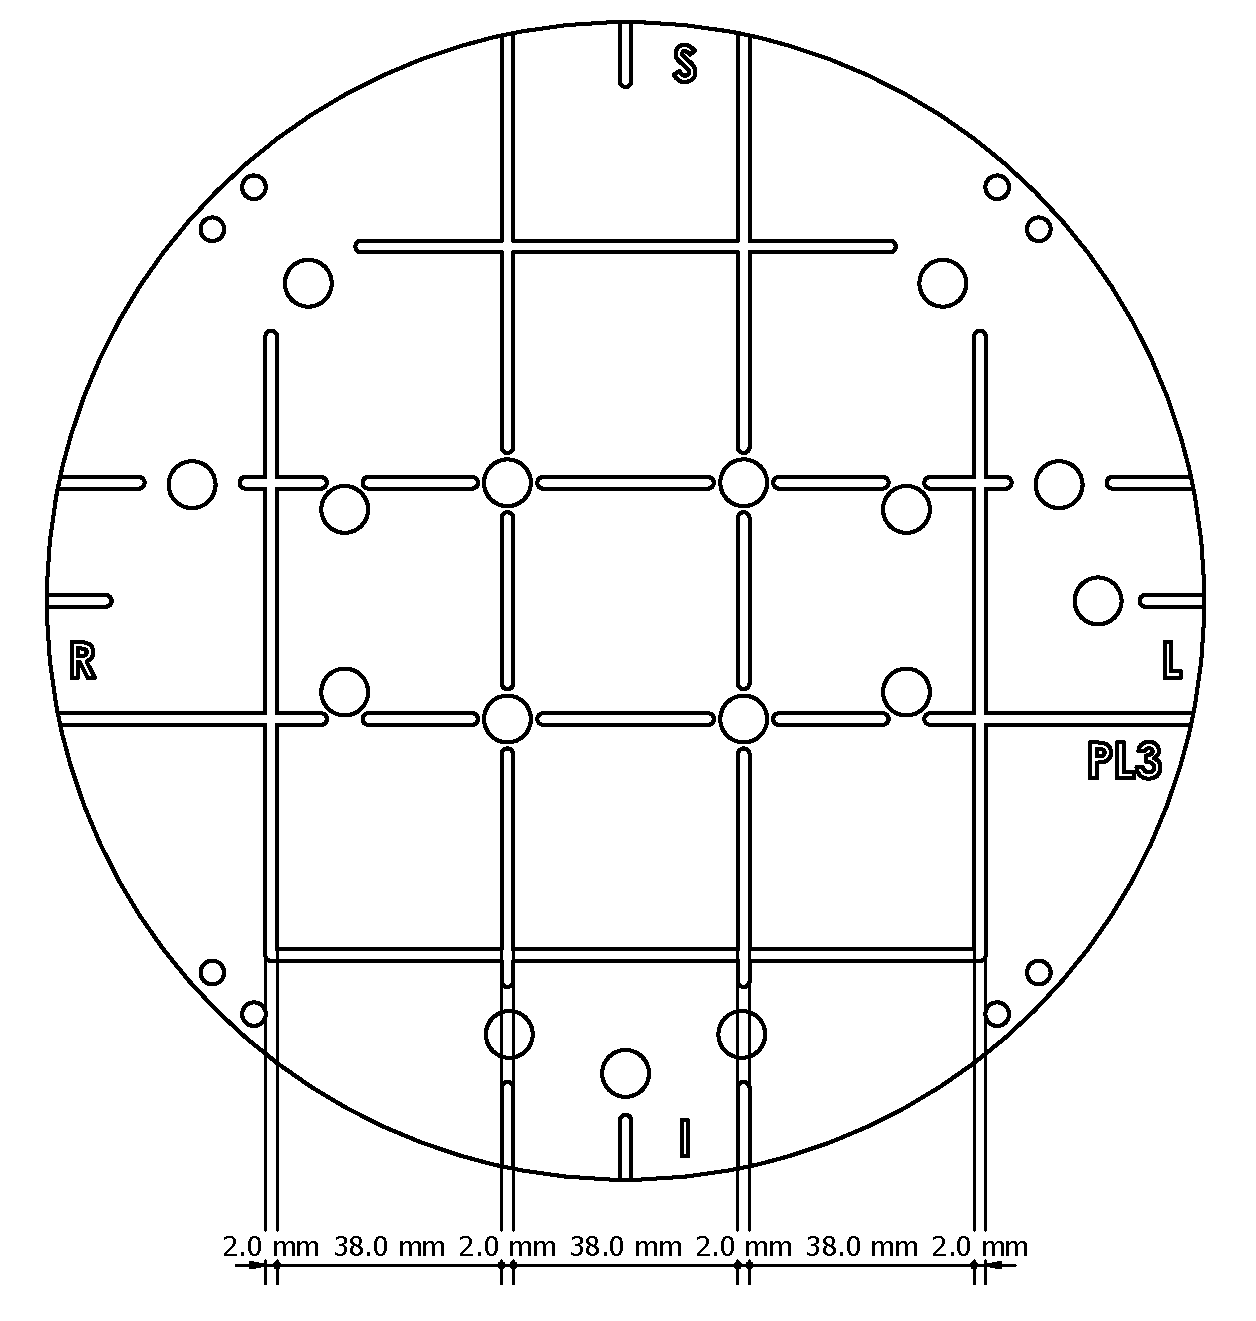
\includegraphics[width=1\textwidth]{T2_Mapping/2D_Blur/Plate_3_Grid_crop.pdf}
	\caption{}
	\label{fig:t2_blur_grid}
\end{subfigure}
\caption{(\subref{fig:t2_phantom_schematic}) A schematic of the $T_2$ spheres in the QalibreMD phantom showing the 14 element \ttwo array and each of the \ttwo values (in ms). (\subref{fig:t2_blur_grid}) A scale drawing of plate three of the QalibreMD system phantom. The grid etched into this plate was used to assess the blurring of each \ttwo mapping sequence.}
\label{fig:t2_nist_phantom}
\end{figure}

The kidneys are highly perfused organs, as such, the effects of fluid flow through the area being imaged should be evaluated. This was achieved using a Gold Standard Phantoms \ac{QASPER} phantom. This phantom comprises of a \ac{MRI} compatible pump with adjustable, continuous, flow rates from 0 m$\ell$/min to 350 m$\ell$/min. The perfusate exits the pump into a series of simulated arterioles before entering a cylinder of porous media designed to simulate a capillary bed. Having travelled through the porous media, the perfusate exits at the centre of the cylinder and is returned to the pump, Figure \ref{fig:t2_flow_phantom_schematic}. 

\begin{figure}[H]
	\centering
	\includegraphics[width=0.5\textwidth]{T2_Mapping/Flow/Flow_schematic.eps}
	%	\missingfigure{Flow phantom schematic}
	\caption{A schematic of the \ac{QASPER} phantom used to quantify the effects of flow upon the \ttwo measurements.}
	\label{fig:t2_flow_phantom_schematic}	
\end{figure}

Both the QalibreMD and \ac{QASPER} phantoms were scanned using a 32-channel head coil. 

\subsection{In-Vivo Data Acquisition}
All data acquired on human subjects was with approval of the local ethics committee and the study was conducted in accordance with the Helsinki Declaration. The subjects gave written, informed consent. Humans were scanned using a 16-channel anterior coil array and 16-channel posterior coil array. The final in-vivo comparison dataset consisted of 5 healthy participants (2 female, 3 male, mean age 31 $\pm$ 8 years).

The final protocol comprised a survey, localisers, dual-echo gradient echo $B_0$ map and \ac{DREAM} $B_1$ map \cite{nehrke_dreamnovel_2012}, and each of the optimised \ttwo mapping sequences. Subjects also had \ttwo-weighted and \tone-weighted structural scans collected to enable segmentation of the whole kidneys, and cortex/medulla respectively \cite{petzold_building_2014, will_automated_2014}, see Chapter \ref{chap:ML}. These \ac{ROI} were then used to calculate the mean \ttwo of each tissue type. 

\subsection{\ttwo Mapping Protocols}
\label{subsec:t2_acq_schemes}
A summary of the acquisition parameters of each \ttwo mapping sequence is shown in Table \ref{tab:t2_sequence_overview}. In-vivo respiratory motion was counteracted via use of respiratory triggering. Each protocol was designed to be  approximately 2-3 minutes (although this will increase when respiratory triggering is used for in-vivo acquisitions) and have matched key parameters such as voxel size and \ac{FOV}. More accurate or higher resolution \ttwo mapping may be possible with longer acquisition times, however as the aim is for this sequence to be used as part of a multiparametric renal protocol, the time constraints of the whole protocol must be considered. 

\begin{table}[H]
	\centering
	\begin{adjustbox}{width=1.0\textwidth, center}
	\begin{tabularx}{1.25\textwidth}{X|X|X|X|X}
		                                                     & Spin Echo - Echo Planar Imaging & Multi-Echo Turbo Spin Echo & Gradient Spin Echo & CPMG \ttwo Preparation - Echo Planar Imaging \\ \hline
		Abbreviation                                         & SE-EPI                          & ME-TSE                     & GraSE              & CPMG \ttwo Prep     \\ \hline
		TE (min:step:max) (ms)                               & 20:10:70                        & 13:13:130                  & 11.2:5.6:173.3     & 0:20:160            \\ \hline
		Number of   echoes                                   & 6                               & 10                         & 30                 & 9                   \\ \hline
		Startup echoes                                       & N/A                             & 0                          & 1                  & N/A                 \\ \hline
		TR (ms)                                              & 5000                            & 3000                       & 3000               & 3000                \\ \hline
		Acquisition Voxel Size   (mm$^3$)                    & 3 $\times$ 3 $\times$ 5         & 3 $\times$ 3 $\times$ 5    &3 $\times$ 3 $\times$ 5 &3 $\times$ 5.65 $\times$ 5\\ \hline
		Reconstruction Voxel Size   (mm$^3$)                 & 3 $\times$ 3 $\times$ 5         & 3 $\times$ 3 $\times$ 5    &3 $\times$ 3 $\times$ 5 &3 $\times$ 3 $\times$ 5\\ \hline
		FoV (mm$^3$)                                         & 288 $\times$ 288 $\times$ 25    & 288 $\times$ 288 $\times$ 25&288 $\times$ 288 $\times$ 25&288 $\times$ 288 $\times$ 25\\ \hline
		Signal   Averages                                    & 2                               & 1                          & 1                  & 1                   \\ \hline
		Packages                                             & 1                               & 1                          & 2                  & 1                   \\ \hline
		Acquisition Mode                                     & Multi Slice                     & Multi Slice                & Multi Slice        & Multiple 2D         \\ \hline
		Fast   Imaging Mode                                  & EPI                             & TSE                        & GraSE              & TFEPI               \\ \hline
		Flip Angle                                           & 90$\degree$                     & 90$\degree$                & 90$\degree$        & 90$\degree$         \\ \hline
		Bandwidth   (Hz)                                     & 40 (Phase), 1787 (Freq)         & 180                        & 405 (Phase), 2268 (Freq) & 113 (Phase), 2845 (Freq)\\ \hline
		SENSE                                                & 2.55                            & 2.55                       & 2.55               & 3                   \\ \hline
		Halfscan                                             & 0.838                           & No                         & No                 & 0.706               \\ \hline
		TSE Factor                                           & N/A                             & 10                         & 30                 & N/A                 \\ \hline
		EPI Factor                                           & 37                              & N/A                        & 3                  & 17                  \\ \hline
		Respiratory Compensation                             & Triggered                       & Triggered                  & Triggered          & Triggered           \\ \hline
		Acquisition Time \scriptsize{(before respiratory compensation)} & 1 min 45 sec                & 1 min 57 sec               & 2 min 6 sec        & 2 min 23 sec  
	\end{tabularx}
	\end{adjustbox}
	\caption{A summary of the acquisition parameters of each of the \ttwo mapping methods compared. \ac{SE}-\ac{EPI}, \ac{ME-TSE} and \ac{GraSE} are standard vendor sequences, whilst the \ac{CPMG} \ttwo prep sequence has been coded specially.}
	\label{tab:t2_sequence_overview}
\end{table}

\subsection{Post Processing}

All post processing was performed using Python 3.7 making use of the \ac{UKAT} \cite{daniel_ukrin_2021, nery_ukrin_2020}. This open source software is specially designed for quantitative renal \ac{MRI}. All curve fitting uses a least squares trust region reflective method to estimate unknown parameters.

\subsubsection{\ttwo Fitting Methods}

The data were fit using a mono-exponential model. Since there are multiple models for fitting noisy data, each of these was evaluated and is illustrated in Figure \ref{fig:t2_fitting_methods}. 

The ``basic fit'' simply takes the signal from each voxel at each \ac{TE} and fits to a monoexponential decay 
\begin{equation}
	S(t) = S_0 \cdot e^{-t/T_2}.
	\label{eq:t2}
\end{equation}
If no noise was present in the data and the sample was a single pure substance i.e. does not exhibit partial voluming effects, this would be the optimum method however, the decreased \ac{SNR} of later \acp{TE} often leads to inaccurate fits. To combat this, the data can be fit to
\begin{equation}
	S(t) = S_0 \cdot e^{-t/T_2} + \epsilon,
	\label{eq:t2_noise}
\end{equation}
where $\epsilon$ represents thermal noise and a baseline in the signal due to long \ttwo compartments; this fitting method is referred to as ``noise fit''. This method is implemented in the software written by \ac{NIST} and distributed with the QalibreMD phantom. Another common method of negating the effects of the low \ac{SNR} of later \ac{TE} is to discard data below a threshold, illustrated in Figure \ref{fig:t2_fitting_methods} at 0.2 AU and referred to as ``discard fit''. Finally, a combination of both noise estimation and discarding can be performed (``discard and noise fit''). All four of these fitting methods will be compared.

\begin{figure}[H]
	\centering
	\includegraphics[width=0.7\textwidth]{T2_Mapping/fitting_methods.pdf}
	\caption{The four fitting methods used to estimate \ttwo of simulated data shown here with \ttwo=50 ms and mean \ac{SNR}=23. Simulated data is used here only for illustration, all evaluations of fitting methods were performed on true data collected from the QalibreMD phantom.}
	\label{fig:t2_fitting_methods}	
\end{figure}

These fitting methods can either be applied on a voxel-by-voxel basis to generate spatial maps or, the signal from all voxels in an \ac{ROI} with a single \ttwo can be averaged at each \ac{TE} with parameters being fit to the subsequent mean signal. 

\subsection{Assessment of Data}

\subsubsection{Quantifying Accuracy}
Using the QalibreMD phantom, the quantitative accuracy of each of the sequences was assessed. A voxel-by-voxel \ttwo map was calculated for each sequence, \acp{ROI} were then defined for each of the spheres in the \ttwo array, Figure \ref{fig:t2_phantom_loc}, and the mean \ttwo within each sphere calculated. The estimated values of \ttwo were compared to the ground truth literature values and their discrepancy assessed over both the full range of \ttwo values in the array (5 ms – 650 ms) and the range of \ttwo reported in the kidneys (40 ms – 200 ms) \cite{wolf_magnetic_2018}. Accuracy was summarised over these ranges using \ac{MPE} defined as 
\begin{equation}
	\textup{MPE} = \frac{1}{N}\sum_{n}^{i=1}\left|  \frac{t_{2\; i}^{\textup{ground truth}} - t_{2\; i}^{\textup{estimate}}}{t_{2\; i}^{\textup{ground truth}}}\right| \cdot 100.
	\label{eq:t2_MPE}
\end{equation}
In addition to the four protocols that can be applied in-vivo, the \ac{NIST} recommended ME-SE scheme was also used to validate that the \ttwo values of the phantom used in this study were in agreement with the literature values.

\begin{figure}[H]
	\centering
	\includegraphics[width=0.5\textwidth]{T2_Mapping/Phantom_Example/Localiser_multi.eps}
	\caption{The $T_2$ spheres inside the QalibreMD phantom.}
	\label{fig:t2_phantom_loc}	
\end{figure}

\subsubsection{Effects of Flow}
To investigate the effects of flow upon \ttwo measurements, the \ac{QASPER} phantom was used. The porous media was imaged using each sequence over the full range of flow rates the phantoms pump can deliver. \ttwo maps are calculated and the mean \ttwo calculated to evaluate the robustness of each sequence to variations in perfusion.

\newpage
\subsubsection{Blurring}
The amount of blurring of an image is different for each sequence and can dramatically effect the readability of an image and ultimately its clinical utility. In \ac{MRI} the amount and characteristics of the blur is usually spatially invariant, that is to say, if a voxel in the centre of an image is blurred over its five neighbouring voxels in the phase encode direction, a voxel at the edge of the image would also be blurred over its five neighbouring voxels. The degree of blurring produced by each of the sequences outlined in Section \ref{subsec:t2_acq_schemes} was quantified.

The observed image, $h$, can be modelled as an ideal, unblurred signal, $f$ distorted by a filter, $g$, Figure \ref{fig:t2_1d_blur}. This distorting filter is known as the \ac{PSF} and is the theoretical signal produced when imaging an infinitely small point source object or, in practice, the blurring observed in the imaging system when an object much smaller than the systems resolving power is imaged. In a spatially invariant system, such as \ac{MRI}, the recorded signal is simply a convolution of the true signal and the \ac{PSF} i.e. $f \ast g = h$. By fitting a Gaussian to the \ac{PSF} the degree of blurring in the image can be quantified \cite{chaimow_more_2017, chaimow_more_2017-1}. 
\begin{figure}[H]
	\centering
	\includegraphics[width=0.8\textwidth]{T2_Mapping/1D_Blur/1d_conv.eps}
	\caption{The convolution of the ideal signal, $f$, and the \ac{PSF}, $g$, produces the measured signal, $h$.}
	\label{fig:t2_1d_blur}	
\end{figure}

A 3 mm deep, 2 mm thick, grid etched into one of the plastic plates of the QalibreMD phantom, Figure \ref{fig:t2_blur_grid}, was imaged using each of the \ttwo mapping methods with an echo time of 20 ms. A 0.5 mm$^3$ isotropic structural scan was also collected. The thickness of the grid is smaller than the imaging resolution of the \ttwo mapping sequences and the resolution of the structural scan is much greater than the resolution of the \ttwo mapping scans, therefore the structural scan can be seen as an approximation of the ideal image produced by each \ttwo mapping method. As shown in Figure \ref{fig:t2_2d_blur}, this allows a deconvolution of the \ac{PSF} from the \ttwo mapping scans and, by fitting a Gaussian to the line profiles through the centre of the \ac{PSF} in each direction (indicated by the blue and orange dashed lines on the estimated \ac{PSF}), an estimate of the \ac{FWHM} of the \ac{PSF}. Quoted values are the maximum \ac{PSF} of each of the in-plane directions as this is the limiting factor in the readability of an image, for the example in Figure \ref{fig:t2_2d_blur}, the quoted \ac{PSF} would be 9.5 $\pm$ 0.2 mm.

\begin{figure}[H]
	\centering
	\includegraphics[width=1\textwidth]{T2_Mapping/2D_Blur/Example/2D_Blur.eps}
	\caption{An overview of the estimation of the \ac{PSF}. For this illustration the \ttwo-weighted data has had additional blur added to make the effect of each processing step clearer.}
	\label{fig:t2_2d_blur}	
\end{figure}

\subsubsection{In-Vivo}

Using the \tone-weighted structural scans \ac{ROI} were defined for both the renal cortex and medulla of each subject. These \ac{ROI} were then used to calculate the mean and standard deviation \ttwo for each tissue type of each subject. Histogram analysis was also performed to interrogate the distribution of \ttwo within each tissue. \ttwo maps were qualitatively assessed for their readability.

\newpage

\section{Results}

\subsection{Verification of Phantom Accuracy}
To ascertain the accuracy of the scanner and QalibreMD phantom, the \ac{NIST} recommended ME-SE protocol was first performed. This verifies that the phantom has been manufactured correctly, that the scanner produces acceptable results when running a standardised protocol and provides context to the accuracies of the in-vivo sequences i.e. understanding how much accuracy has been sacrificed to make the protocol practical for renal imaging. Fitting is shown using the basic fit as this resulted in the closest fit to literature values, however all fitting methods were evaluated, with results included in Appendix \ref{app:t2_fitting_nist}. The only noteworthy variances between fitting methods was observed for the spheres of very short \ttwo.

When comparing the \ttwo calculated to the literature values supplied with the phantom, Figure \ref{fig:t2_nist}, the \ac{MPE} over the full range of spheres was $-5~\pm~7~\%$, and over the range of \ttwo expected in the kidneys was $-6~\pm~3~\%$ where values are expressed as mean percentage error over the range of spheres $\pm$ the standard deviation in percentage error over the range of spheres. 

\begin{figure}[H]
	\centering
	\begin{subfigure}[c]{0.47\textwidth}
		\centering
		\includegraphics[width=1\textwidth]{T2_Mapping/Phantom_cor/NIST_all.pdf}
		\caption{}
		\label{fig:t2_nist_cor}
	\end{subfigure}
	\hfill
	\begin{subfigure}[c]{0.47\textwidth}
		\centering
		\includegraphics[width=1\textwidth]{T2_Mapping/Phantom_cor/NIST_re_all.pdf}
		\caption{}
		\label{fig:t2_nist_re}
	\end{subfigure}
	\caption{\ttwo measured using the standardised \ac{NIST} protocol compared to the reference \ttwo from the manufacturer. (\subref{fig:t2_nist_cor}) shows the correlation and (\subref{fig:t2_nist_re}) shows the relative error between these values.}
	\label{fig:t2_nist}
\end{figure}
\subsection{Fitting Methods}
\label{subsec:t2_fitting_methods_results}
Each fitting method was tested using data acquired on the QalibreMD phantom and in-vivo. A full breakdown of the accuracy of each fitting method, applied to each sequence, over different ranges of \ttwo can be seen in Table \ref{tab:t2_phantom_fitting_methods} and Figure \ref{fig:t2_in_vivo_fitting_methods}. Figures showing the accuracy and \ac{MPE} of each sequence and fitting method are included in Appendix \ref{app:t2_fitting_renal}. The QalibreMD analysis software for the phantom calculates the mean signal from each sphere then fits this to a \ttwo decay, resulting in a quicker and more accurate measurement of the homogeneous \ttwo of each sphere \cite{mristandards_mristandardsphantomviewer_2020}. Due to the heterogeneity within the kidneys, this method could not be applied in-vivo and as such, the accuracy of the sequences and fitting methods was evaluated by performing a voxel-by-voxel fit, then calculating the mean \ttwo from an \ac{ROI} of each sphere in the resulting map.

\begin{table}[H]
	\centering
	\begin{adjustbox}{width=1.0\textwidth, center}
	\begin{tabularx}{1.4\textwidth}{X|X|X|X|X|X|X|X|X|X}
		\ttwo   Range            & \multicolumn{4}{c|}{MPE   (5 ms – 650 ms) (\%)}                         & \multicolumn{5}{c}{MPE   (40 ms – 200 ms) (\%)}              \\ \hline
		Fitting   Method      & Basic     & Noise     & Discard   & Discard   and Noise & \multicolumn{2}{l|}{Basic}     & Noise      & Discard   & Discard   and Noise \\ \hline
		SE-EPI                & 36 $\pm$  34   & 202 $\pm$  437 & 33 $\pm$  34   & 238 $\pm$  463           & \multicolumn{2}{l|}{8 $\pm$  5}     & 32 $\pm$  42    & 22 $\pm$  8    & 31 $\pm$  42             \\ \hline
		ME-TSE                & 38   $\pm$  31 & 13   $\pm$  16 & 41   $\pm$  35 & 35   $\pm$  36           & \multicolumn{2}{l|}{23   $\pm$  13} & 14   $\pm$  3   & 15   $\pm$  13 & 13   $\pm$  4            \\ \hline
		GraSE                 & 32 $\pm$  29   & 23 $\pm$  27   & 26 $\pm$  28   & 33 $\pm$  37             & \multicolumn{2}{l|}{15 $\pm$  4}    & 11 $\pm$  5     & 13 $\pm$  4    & 9 $\pm$  7               \\ \hline
		CPMG   \ttwo Prep        & 18   $\pm$  15 & 30   $\pm$  53 & 20   $\pm$  18 & 28   $\pm$  28           & \multicolumn{2}{l|}{11   $\pm$  1}  & 8   $\pm$  5    & 11   $\pm$  1  & 6   $\pm$  5             \\ \hline \hline
		Mean   over sequences & 31   $\pm$  8  & 67   $\pm$  90 & 30   $\pm$  9  & 83   $\pm$  103          & \multicolumn{2}{l|}{14   $\pm$  7}  & 16   $\pm$  11  & 14   $\pm$  36 & 15   $\pm$  11          
	\end{tabularx}
	\end{adjustbox}
	\caption{\ac{MPE} when measuring \ttwo of the QalibreMD phantom over different ranges using each sequence and fitting method. 5 ms – 650 ms is the full range of \ttwo available in the phantom and 40 ms – 200 ms is the range of \ttwo reported in the kidneys. Values are expressed as mean percentage error of the spheres within the specified range of \ttwo $\pm$ the standard deviation of percentage error over the spheres within the specified range of \ttwo.}
	\label{tab:t2_phantom_fitting_methods}
\end{table}

\begin{figure}[H]
	\centering
	\begin{subfigure}[c]{0.47\textwidth}
		\centering
		\includegraphics[width=1\textwidth]{T2_Mapping/Fitting_methods_invivo/basic.eps}
		\caption{Basic fit}
		\label{fig:t2_in_vivo_fitting_methods_basic}
	\end{subfigure}
	\hfill
	\begin{subfigure}[c]{0.47\textwidth}
		\centering
		\includegraphics[width=1\textwidth]{T2_Mapping/Fitting_methods_invivo/noise.eps}
		\caption{Noise fit}
		\label{fig:t2_in_vivo_fitting_methods_noise}
	\end{subfigure}

	\vskip\baselineskip
	\begin{subfigure}[c]{0.47\textwidth}
		\centering
		\includegraphics[width=1\textwidth]{T2_Mapping/Fitting_methods_invivo/discard.eps}
		\caption{Discard fit}
		\label{fig:t2_in_vivo_fitting_method_discards}
	\end{subfigure}
	\hfill
	\begin{subfigure}[c]{0.47\textwidth}
		\centering
		\includegraphics[width=1\textwidth]{T2_Mapping/Fitting_methods_invivo/noise_discard.eps}
		\caption{Discard and noise fit}
		\label{fig:t2_in_vivo_fitting_methods_noise_discard}
	\end{subfigure}
	\vskip\baselineskip
	\begin{subfigure}[c]{0.6\textwidth}
		\centering
		\includegraphics[width=1\textwidth]{T2_Mapping/Fitting_methods_invivo/grase_fitting_methods_joy.pdf}
		\caption{}
		\label{fig:t2_in_vivo_fitting_methods_hist}
	\end{subfigure}
	\caption{(\subref{fig:t2_in_vivo_fitting_methods_basic}-\subref{fig:t2_in_vivo_fitting_methods_noise_discard}) \ttwo maps generated using each of the fitting methods for the \ac{GraSE} sequence and (\subref{fig:t2_in_vivo_fitting_methods_hist}) histograms of \ttwo values within the renal cortex, renal medulla, liver and spleen. The reduction in longer \ttwo values when fit with a noise term observed in the phantom can be seen here in the large decrease in \ttwo of the kidneys, while the spleen and liver only decrease a small amount. Discarding has relatively little effect on the kidneys but does slightly increase the variance in \ttwo within each \ac{ROI}.}
	\label{fig:t2_in_vivo_fitting_methods}
\end{figure}


The noise fit results in an increase in accuracy compared to the basic fit when measuring the \ttwo of the shortest \ttwo spheres, especially for sequences with a short echo spacing where the majority of echoes in the signal are after the sphere has fully relaxed back to its baseline noise level. This increase in accuracy for short \ttwo is at the expense of the accuracy of the long \ttwo spheres. The combination of decreased dynamic range and an extra parameter to optimise resulted in an inaccurate characterisation of these spheres, especially of the \ac{SE}-\ac{EPI} sequence due to the short final echo time and thus lower dynamic range. This can be observed in Figure \ref{fig:t2_in_vivo_fitting_methods_hist} where the variance in \ttwo within the liver is decreased when using the noise fit compared to the basic fit, however the variance of the longer \ttwo values in the kidneys has increased. In the range of \ttwo reported in the kidney, the noise fit increased the average error over the four sequences. 

The discard fit requires an empirical threshold to be chosen. If chosen correctly, this results in a slightly improved accuracy however, if the threshold was not correctly chosen the accuracy of \ttwo was compromised. While optimising the threshold is trivial when the known reference values are available, this is more difficult in-vivo and therefore, given the increase in accuracy was marginal and only effected spheres of short \ttwo, consistent results were deemed preferable. The combination of discard and noise fit resulted in a decreased accuracy from the basic fit. Spheres that benefited from the additional noise term relax to their baseline noise quickly, however by discarding these echoes, the estimate of noise becomes inaccurate and thus so does the estimate of \ttwo. It was therefore concluded that a basic fit should be used for all subsequent renal data.

\subsection{Phantom Verification}

\subsubsection{Accuracy}

Each sequence was used to image the \ttwo array in the QalibreMD phantom. Figure \ref{fig:t2_phantom_cor} shows the measured \ttwo plot against the reference \ttwo for each method. All methods struggle to accurately measure the very short \ttwo spheres in the array, with the \ac{CPMG} \ttwo prep method performing best. The \ac{SE}-\ac{EPI} method overestimates short \ttwo spheres due to the first \ac{TE} being sampled at 20~ms but is also underestimating long \ttwo because of its small range in \ac{TE}. When considering only the spheres with physiologically similar \ttwo to the kidneys, the \ac{SE}-\ac{EPI} method is the most accurate with the \ac{GraSE} and \ac{CPMG} \ttwo prep delivering similar results. This is mirrored by the \ac{MPE} shown in Table \ref{tab:t2_phantom_acquisition_methods}. Example \ttwo maps of the phantoms \ttwo array imaged with each sequence are shown in Figure \ref{fig:t2_phantom_maps}.

\begin{figure}[H]
	\centering
	\begin{subfigure}[c]{0.47\textwidth}
		\centering
		\includegraphics[width=1\textwidth]{T2_Mapping/Phantom_cor/basic_fit_full.pdf}
		\caption{}
		\label{fig:t2_phantom_cor_full}
	\end{subfigure}
	\hfill
	\begin{subfigure}[c]{0.47\textwidth}
		\centering
		\includegraphics[width=1\textwidth]{T2_Mapping/Phantom_cor/basic_fit_kidney.pdf}
		\caption{}
		\label{fig:t2_phantom_cor_kidney}
	\end{subfigure}
	\vfill
		\begin{subfigure}[c]{0.47\textwidth}
		\centering
		\includegraphics[width=1\textwidth]{T2_Mapping/Phantom_cor/basic_re_full.pdf}
		\caption{}
		\label{fig:t2_phantom_re_full}
	\end{subfigure}
	\hfill
	\begin{subfigure}[c]{0.47\textwidth}
		\centering
		\includegraphics[width=1\textwidth]{T2_Mapping/Phantom_cor/basic_re_kidney.pdf}
		\caption{}
		\label{fig:t2_phantom_re_kidney}
	\end{subfigure}
	\caption{\ttwo measured using each acquisition method compared to the reference \ttwo from literature. (\subref{fig:t2_phantom_cor_full}) The full range of \ttwo spheres is shown on logarithmic axis with the range of \ttwo reported in the kidneys shaded in red (\subref{fig:t2_phantom_cor_kidney}) The spheres with \ttwo in the range of the kidneys are shown on linear axis. (\subref{fig:t2_phantom_re_full}) and (\subref{fig:t2_phantom_re_kidney}) show the relative error of each sphere for the full and renal range of spheres respectively.}
	\label{fig:t2_phantom_cor}
\end{figure}

\begin{table}[H]
	\centering
	\begin{tabularx}{1\textwidth}{X|X|X}
		Acquisition   Method & MPE   (5 ms – 650 ms) (\%) & MPE   (40 ms – 200 ms) (\%) \\ \hline
		SE-EPI               & 36 $\pm$ 34                    & 8   $\pm$ 5                     \\ \hline
		ME-TSE               & 38   $\pm$ 31                  & 23 $\pm$ 13                     \\ \hline
		GraSE                & 32 $\pm$ 29                    & 15   $\pm$ 4                    \\ \hline
		CPMG   \ttwo Prep       & 18   $\pm$ 15                  & 11   $\pm$ 1                   
	\end{tabularx}
	\caption{\ac{MPE} when measuring \ttwo of the QalibreMD phantom over different ranges using each sequence. 5 ms – 650 ms is the full range of \ttwo available in the phantom and 40 ms – 200 ms is the range of \ttwo expected in the kidneys. Values are expressed as mean percentage error of the spheres within the specified range of \ttwo $\pm$ the standard deviation of percentage error over the spheres within the specified range of \ttwo.}
	\label{tab:t2_phantom_acquisition_methods}
\end{table}

\begin{figure}[H]
	\centering
	\begin{subfigure}[c]{0.47\textwidth}
		\centering
		\includegraphics[width=1\textwidth]{T2_Mapping/Phantom_maps/SE.pdf}
		\caption{\ac{SE}-\ac{EPI}}
		\label{fig:t2_phantom_map_se}
	\end{subfigure}
	\hfill
	\begin{subfigure}[c]{0.47\textwidth}
		\centering
		\includegraphics[width=1\textwidth]{T2_Mapping/Phantom_maps/ME.pdf}
		\caption{\ac{ME-TSE}}
		\label{fig:t2_phantom_map_me_tse}
	\end{subfigure}
	
	\vskip\baselineskip
	\begin{subfigure}[c]{0.47\textwidth}
		\centering
		\includegraphics[width=1\textwidth]{T2_Mapping/Phantom_maps/GraSE.pdf}
		\caption{\ac{GraSE}}
		\label{fig:t2_phantom_map_grase}
	\end{subfigure}
	\hfill
	\begin{subfigure}[c]{0.47\textwidth}
		\centering
		\includegraphics[width=1\textwidth]{T2_Mapping/Phantom_maps/CPMG.pdf}
		\caption{\ac{CPMG} \ttwo Prep}
		\label{fig:t2_phantom_map_cpmg_t2_prep}
	\end{subfigure}
	\vskip\baselineskip
	\begin{subfigure}[c]{0.35\textwidth}
		\centering
		\includegraphics[width=1\textwidth]{T2_Mapping/Phantom_Example/T2_Spheres.eps}
		\caption{Literature Values}
		\label{fig:t2_phantom_map_true}
	\end{subfigure}
	\caption{\ttwo maps of the QaliberMD system phantom \ttwo array generated using each sequence.}
	\label{fig:t2_phantom_maps}
\end{figure}

\subsubsection{Sensitivity to Flow}

To assess the sensitivity of each of the \ttwo mapping schemes to flow, the simulated capillary bed of the flow phantom was imaged with the perfusate pumped at rates from 0 to 350 m$\ell$/min. The absolute change in measured \ttwo is shown in Figure \ref{fig:t2_flow_abs} and the change in \ttwo as a percentage of \ttwo measured when the pump was turned off is shown in Figure \ref{fig:t2_flow_percent}. The \ttwo of the perfusate is relatively long and as such the inaccuracies measuring long \ttwo observed in the static phantom (Figure \ref{fig:t2_phantom_cor_full} and Figure \ref{fig:t2_phantom_re_full}) manifest themselves here. This causes a large range in \ttwo even when the pump is turned off. In Figure \ref{fig:t2_flow_percent} the \ac{SE}-\ac{EPI} sequence can be seen to be most sensitive to perfusion due to its largest deviation as flow rate increased, the \ac{GraSE} sequence produced the minimum proportional change in \ttwo as the rate perfusate was pumped through the capillary bed was increased.
\begin{figure}[H]
	\centering
	\begin{subfigure}[c]{0.47\textwidth}
		\centering
		\includegraphics[width=1\textwidth]{T2_Mapping/Flow/flow_abs.pdf}
		\caption{}
		\label{fig:t2_flow_abs}
	\end{subfigure}
	\hfill
	\begin{subfigure}[c]{0.47\textwidth}
		\centering
		\includegraphics[width=1\textwidth]{T2_Mapping/Flow/flow_per.pdf}
		\caption{}
		\label{fig:t2_flow_percent}
	\end{subfigure}
	\caption{The effects of flow on measurements of \ttwo using each method. Points have been slightly staggered on the $x$-axis to aide the visibility of error bars. (\subref{fig:t2_flow_abs}) Absolute measured \ttwo. (\subref{fig:t2_flow_percent}) Change in \ttwo as a percentage of \ttwo measured at rest for each sequence. Error bars are derived from the standard deviation within the \ac{ROI}.}
	\label{fig:t2_flow}
\end{figure}

The flow rate is measured at the pump, therefore the perfusate will not be travelling at the reported rate through the capillary bed. To quantify the movement of the perfusate using techniques widely available in the kidneys, \ac{ADC} maps of the capillary bed were calculated at each flow rate. More information on \ac{ADC} mapping is given in Sections \ref{subsec:theory_diffusion} and \ref{subsec:ex_adc}. The protocol used here was a monopolar \ac{SE}-\ac{EPI} scheme with fixed diffusion time i.e. different b-values were achieved solely by modulating the gradient strength. b-values acquired were 0, 5, 15, 30, 45, 60, 75, 400 and 600 s/mm$^2$. Using this scheme, \ac{ADC} in the capillary bed with different perfusate flow rates was calculated, Figure \ref{fig:t2_flow_adc}. 

\begin{figure}[H]
	\centering
	\includegraphics[width=0.6\textwidth]{T2_Mapping/Flow/flow_adc.pdf}
	\caption{Changes in ADC as the rate at which perfusate is pumped through the simulated capillary bed is increased. Error bars are derived from the standard deviation within the \ac{ROI}.}
	\label{fig:t2_flow_adc}	
\end{figure} 

\subsubsection{Image Blurring}

Each sequence was slightly modified to contain an acquisition with a \ac{TE} of 20 ms to ensure a constant \ttwo weighting across techniques and this was used to image the orthogonal grid in the QalibreMD phantom, Figure \ref{fig:t2_blur_grid}. A high-resolution structural scan was then used to deconvolve an estimate of the \ac{PSF} from each of the \ttwo-weighted images allowing the \ac{FWHM} to be estimated, Table \ref{tab:t2_phantom_blur}. Examples of the central slice of the grid imaged with each method are shown in Figure \ref{fig:t2_phantom_blur}. 

\begin{table}[H]
	\centering
	\begin{tabular}{l|l}
		Acquisition   Method & PSF FWHM (mm)        \\ \hline
		SE-EPI               & 4.80   $\pm$ 0.18    \\ \hline
		ME-TSE               & 4.20 $\pm$ 0.14      \\ \hline
		GraSE                & 4.26   $\pm$ 0.12    \\ \hline
		CPMG   \ttwo Prep    & 6.48   $\pm$ 0.33                    
	\end{tabular}
	\caption{The \ac{FWHM} of the estimated \ac{PSF} for each acquisition method. Uncertainty is calculated from the confidence in the Gaussian fit.}
	\label{tab:t2_phantom_blur}
\end{table}

\begin{figure}[H]
	\centering
	\begin{subfigure}[c]{0.30\textwidth}
		\centering
		\includegraphics[width=1\textwidth]{T2_Mapping/Phantom_blur/gold.png}
		\caption{Structural Scan}
		\label{fig:t2_phantom_blur_gold}
	\end{subfigure}
	\hfill
	\begin{subfigure}[c]{0.30\textwidth}
		\centering
		\includegraphics[width=1\textwidth]{T2_Mapping/Phantom_blur/se.png}
		\caption{\ac{SE}-\ac{EPI}}
		\label{fig:t2_phantom_blur_se}
	\end{subfigure}
	\hfill
	\begin{subfigure}[c]{0.30\textwidth}
		\centering
		\includegraphics[width=1\textwidth]{T2_Mapping/Phantom_blur/me.png}
		\caption{\ac{ME-TSE}}
		\label{fig:t2_phantom_blur_me}
	\end{subfigure}
	\vskip\baselineskip
	\hfill
	\begin{subfigure}[c]{0.30\textwidth}
		\centering
		\includegraphics[width=1\textwidth]{T2_Mapping/Phantom_blur/grase.png}
		\caption{\ac{GraSE}}
		\label{fig:t2_phantom_blur_grase}
	\end{subfigure}
	\hbox to 6.3mm{}% !!
	\begin{subfigure}[c]{0.30\textwidth}
		\centering
		\includegraphics[width=1\textwidth]{T2_Mapping/Phantom_blur/cpmg.png}
		\caption{\ac{CPMG} \ttwo Prep}
		\label{fig:t2_phantom_blur_cpmg}
	\end{subfigure}
	\caption{Examples of the orthogonal grid imaged with a \ac{TE} of 20 ms using each \ttwo mapping sequence and the high-resolution structural scan used as the gold standard to deconvolve from each \ttwo-weighted scan.}
	\label{fig:t2_phantom_blur}
\end{figure}

Both the \ac{SE}-\ac{EPI} and \ac{CPMG} \ttwo prep \ac{EPI} sequences suffer from significant image distortions due to their \ac{EPI} readout with the \ac{ME-TSE} and \ac{GraSE} both producing similar image quality and a comparable width of \ac{PSF}.

\subsection{Summary of Evaluation of \ttwo Mapping Sequences on Phantoms}
The phantom evaluation of each sequence is summarised in Figure \ref{fig:t2_summary}. This figure combines the quantitative accuracy of \ttwo within the range of the kidneys, the sensitivity to fluid motion and blurring characteristics of each sequence. The \ac{GraSE} and \ac{CPMG} \ttwo prep sequences produce the most accurate results, however the \ac{GraSE} has a much smaller \ac{PSF}.

\begin{figure}[H]
	\centering
	\includegraphics[width=0.7\textwidth]{T2_Mapping/summary.pdf}
	\caption{A summary of the quantitative accuracy, sensitivity to flow and degree of blurring observed for each \ttwo mapping sequence when evaluated on phantoms.}
	\label{fig:t2_summary}	
\end{figure}
\subsection{In-Vivo}

Having assessed each of the sequences, five healthy volunteers were then imaged using all four methods. Example in-vivo multi echo data and resulting \ttwo maps are shown in Figures \ref{fig:t2_in_vivo_raw} and \ref{fig:t2_in_vivo_maps} respectively. The measured \ttwo using the \ac{SE}-\ac{EPI} method is much lower than that measured using the other three methods. The \ac{GraSE} scheme shows the largest contrast between cortex and medulla while the \ac{CPMG} \ttwo prep suffers from image artefacts with the largest amount of blurring as measured on the phantom.

\begin{figure}[H]
	\centering
	\begin{subfigure}[c]{0.7\textwidth}
		\centering
		\includegraphics[width=0.8\textwidth]{T2_Mapping/Invivo/Raw_Data_SE.eps}
		\caption{\ac{SE}-\ac{EPI}}
		\label{fig:t2_in_vivo_raw_se}
	\end{subfigure}
	\vskip\baselineskip
	\begin{subfigure}[c]{0.7\textwidth}
		\centering
		\includegraphics[width=0.8\textwidth]{T2_Mapping/Invivo/Raw_Data_ME.eps}
		\caption{\ac{ME-TSE}}
		\label{fig:t2_in_vivo_raw_me}
	\end{subfigure}
	\vskip\baselineskip
	\begin{subfigure}[c]{0.7\textwidth}
		\centering
		\includegraphics[width=0.8\textwidth]{T2_Mapping/Invivo/Raw_Data_GraSE.eps}
		\caption{\ac{GraSE}}
		\label{fig:t2_in_vivo_raw_grase}
	\end{subfigure}
	\vskip\baselineskip
	\begin{subfigure}[c]{0.7\textwidth}
		\centering
		\includegraphics[width=0.8\textwidth]{T2_Mapping/Invivo/Raw_Data_T2_Prep.eps}
		\caption{\ac{CPMG} \ttwo Prep}
		\label{fig:t2_in_vivo_raw_t2_prep}
	\end{subfigure}
	\caption{Example in-vivo multi echo data using each of the \ttwo mapping sequences.}
	\label{fig:t2_in_vivo_raw}
\end{figure}
	
\begin{figure}[H]
	\centering
	\begin{subfigure}[c]{0.47\textwidth}
		\centering
		\includegraphics[width=0.9\textwidth]{T2_Mapping/Invivo/se.eps}
		\caption{\ac{SE}-\ac{EPI}}
		\label{fig:t2_in_vivo_map_se}
	\end{subfigure}
	\hfill
	\begin{subfigure}[c]{0.47\textwidth}
		\centering
		\includegraphics[width=0.9\textwidth]{T2_Mapping/Invivo/me.eps}
		\caption{\ac{ME-TSE}}
		\label{fig:t2_in_vivo_map_me_tse}
	\end{subfigure}
	
	\vskip\baselineskip
	\begin{subfigure}[c]{0.47\textwidth}
		\centering
		\includegraphics[width=0.9\textwidth]{T2_Mapping/Invivo/grase.eps}
		\caption{\ac{GraSE}}
		\label{fig:t2_in_vivo_map_grase}
	\end{subfigure}
	\hfill
	\begin{subfigure}[c]{0.47\textwidth}
		\centering
		\includegraphics[width=0.9\textwidth]{T2_Mapping/Invivo/cpmg.eps}
		\caption{\ac{CPMG} \ttwo Prep}
		\label{fig:t2_in_vivo_map_cpmg_t2_prep}
	\end{subfigure}
	\vskip\baselineskip
	\begin{subfigure}[c]{0.47\textwidth}
		\centering
		\includegraphics[width=0.9\textwidth]{T2_Mapping/Invivo/b0.eps}
		\caption{$B_0$}
		\label{fig:t2_in_vivo_map_b0}
	\end{subfigure}
	\hfill
	\begin{subfigure}[c]{0.47\textwidth}
		\centering
		\includegraphics[width=0.9\textwidth]{T2_Mapping/Invivo/b1.eps}
		\caption{$B_1$}
		\label{fig:t2_in_vivo_map_b1}
	\end{subfigure}
	\vskip\baselineskip
	\begin{subfigure}[c]{0.47\textwidth}
		\centering
		\includegraphics[width=.6\textwidth]{T2_Mapping/Invivo/T1W.png}
		\caption{\tone-weighted structural}
		\label{fig:t2_in_vivo_t1w}
	\end{subfigure}
	\hfill
	\begin{subfigure}[c]{0.47\textwidth}
		\centering
		\includegraphics[width=.6\textwidth]{T2_Mapping/Invivo/T2W.png}
		\caption{\ttwo-weighted structural}
		\label{fig:t2_in_vivo_t2w}
	\end{subfigure}
	\caption{Example in-vivo maps generated using each of the sequences and the associated $B_0$ and $B_1$ maps used for quality control and structural scans used for segmentation.}
	\label{fig:t2_in_vivo_maps}
\end{figure}

\ac{ROI} for the cortex and medulla were defined from the \tone-weighted structural scan (Figure \ref{fig:t2_in_vivo_t1w}) and these \ac{ROI} used to calculate the mean \ttwo for the renal cortex and medulla using each mapping method. The mean across the five subjects is shown in Figure \ref{fig:t2_in_vivo_t2_bar}. Additionally the \ac{CoV}, defined as standard deviation upon the mean, between subjects was calculated to assess the repeatability of each measure, Figure~\ref{fig:t2_in_vivo_cov_bar}.

\begin{figure}[H]
	\centering
	\begin{subfigure}[c]{0.47\textwidth}
		\centering
		\includegraphics[width=1\textwidth]{T2_Mapping/Invivo/bar.pdf}
		\caption{}
		\label{fig:t2_in_vivo_t2_bar}
	\end{subfigure}
	\hfill
	\begin{subfigure}[c]{0.47\textwidth}
		\centering
		\includegraphics[width=1\textwidth]{T2_Mapping/Invivo/bar_cov.pdf}
		\caption{}
		\label{fig:t2_in_vivo_cov_bar}
	\end{subfigure}
	\caption{(\subref{fig:t2_in_vivo_t2_bar}) Mean cortical and medullary \ttwo values across five subjects measured using each sequence. Error bars are the standard deviation across subjects. (\subref{fig:t2_in_vivo_cov_bar}) The \ac{CoV} between subjects for each sequence.}
	\label{fig:t2_in_vivo_bars}
\end{figure}

To better explore the variation between subjects, histograms of the \ttwo values of each tissue type were generated for each subject, Figure \ref{fig:t2_in_vivo_joy}. A Gaussian was fit to each histogram to calculate the peak and \ac{FWHM} \ttwo for each sequence and tissue type across subjects, Table \ref{tab:t2_hist}.
\begin{figure}[H]
	\centering
	\begin{subfigure}[c]{0.47\textwidth}
		\centering
		\includegraphics[width=1\textwidth]{T2_Mapping/Invivo/seepi_joy.pdf}
		\caption{\ac{SE}-\ac{EPI}}
		\label{fig:t2_in_vivo_joy_se}
	\end{subfigure}
	\hfill
	\begin{subfigure}[c]{0.47\textwidth}
		\centering
		\includegraphics[width=1\textwidth]{T2_Mapping/Invivo/metse_joy.pdf}
		\caption{\ac{ME-TSE}}
		\label{fig:t2_in_vivo_joy_me_tse}
	\end{subfigure}
	
	\vskip\baselineskip
	\begin{subfigure}[c]{0.47\textwidth}
		\centering
		\includegraphics[width=1\textwidth]{T2_Mapping/Invivo/grase_joy.pdf}
		\caption{\ac{GraSE}}
		\label{fig:t2_in_vivo_joy_grase}
	\end{subfigure}
	\hfill
	\begin{subfigure}[c]{0.47\textwidth}
		\centering
		\includegraphics[width=1\textwidth]{T2_Mapping/Invivo/cpmg_t2_prep_joy.pdf}
		\caption{\ac{CPMG} \ttwo Prep}
		\label{fig:t2_in_vivo_joy_cpmg_t2_prep}
	\end{subfigure}
	\caption{Histograms of the \ttwo of cortex and medulla for all subjects and mapping methods.}
	\label{fig:t2_in_vivo_joy}
\end{figure}

\begin{table}[H]
	\centering
	\begin{tabular}{ll|l|l}
		Sequence                         & Tissue  & Peak (ms)  & FWHM (ms) \\ \hline
		\multirow{2}{*}{SE-EPI}          & Cortex  & 74 $\pm$ 4   & 25 $\pm$ 9  \\ \cline{2-4} 
		& Medulla & 61 $\pm$ 4   & 18 $\pm$ 8  \\ \hline
		\multirow{2}{*}{ME-TSE}          & Cortex  & 109 $\pm$ 4  & 18 $\pm$ 8  \\ \cline{2-4} 
		& Medulla & 115 $\pm$ 5  & 19 $\pm$ 4  \\ \hline
		\multirow{2}{*}{GraSE}           & Cortex  & 112 $\pm$ 5  & 17 $\pm$ 1  \\ \cline{2-4} 
		& Medulla & 126 $\pm$ 6  & 22 $\pm$ 8  \\ \hline
		\multirow{2}{*}{CPMG \ttwo Prep} & Cortex  & 109 $\pm$ 5  & 44 $\pm$ 17 \\ \cline{2-4} 
		& Medulla & 130 $\pm$ 11 & 41 $\pm$ 13
	\end{tabular}
	\caption{Peak and \ac{FWHM} of a Gaussian fit to the histogram of each tissue type. Values are expressed as mean and standard deviation across the five subjects.}
	\label{tab:t2_hist}
\end{table}


\newpage

\section{Discussion}

In this chapter, four of the most common \ttwo mapping methods have been evaluated for use in the kidneys; \ac{SE}-\ac{EPI}, \ac{ME-TSE}, \ac{GraSE} and \ac{CPMG} \ttwo prep. These sequences were validated for quantitative accuracy, image quality and sensitivity to flow using phantoms before being used to image five healthy volunteers. Additionally, four different methods of fitting \ttwo maps from the subsequent multi-echo imaging data were compared.

Of the fitting methods explored, the basic fit was deemed the most appropriate over the range of \ttwo within the kidneys. Fitting for a baseline noise term reduced the calculated \ttwo of longer \ttwo tissues because they had not fully recovered before the final \ac{TE} and as such the noise term was over-estimated. This method would be more appropriate for use in tissues with a shorter \ttwo such as the liver or sequences with a very wide range of \ac{TE}. Discarding \ac{TE} with signal below an empirically derived threshold can result in an increased accuracy for short \ttwo tissues but does not improve the accuracy within the range of the kidneys. The discard threshold can be manually defined; however, this leads to potentially inaccurate results if a sub-optimum threshold is chosen, these inaccurate results can be difficult to identify in-vivo with no gold standard to compare against. An alternative to manually setting a threshold is to define a \ac{ROI} over the liver, the signal from the final \ac{TE} is then used to inform the estimation of the discard threshold as, in most cases due to its very short \ttwo, the liver will have fully recovered by the final \ac{TE}. While this method does eliminate the manual aspect of threshold definition between subjects, it requires the additional manual processing step of delineating an additional \ac{ROI} for no increase in accuracy within the kidneys. Discarding low intensity echoes and fitting for noise also produced inferior results to the basic fit. By discarding the late echo times that the fitting method uses to estimate noise, the $\epsilon$ term becomes less accurate and as such, so does \ttwo. It was therefore concluded that the basic fit should be used for renal studies, however, the noise fit should be considered for liver \ttwo measurements.

The only sequence that was able to accurately estimate the \ttwo of the shortest \ttwo spheres of the QalibreMD phantom was the \ac{CPMG} \ttwo prep, Figure \ref{fig:t2_phantom_cor} and Table \ref{tab:t2_phantom_acquisition_methods}. This is able to achieve an effective echo time of 0 ms and thus sample the signal before it has decayed; for other sequences the first echo time can be multiple times the \ttwo of these short spheres and as such the signal has already decayed by a large proportion of its initial signal. Additionally, the \ac{CPMG} sequence is self-correcting for imperfect 180$\degree$ pulses, and thus the longer \ac{TE} are more accurate. It is the very large relative error of the shortest \ttwo spheres (spheres of \ttwo < 20 ms) that leads to the unacceptably large \ac{MPE} in the other sequences over the full range of \ttwo within the phantom, Figure \ref{fig:t2_phantom_re_full}. Both the \ac{ME-TSE} and \ac{GraSE} yield similar accuracies over the range of \ttwo seen in the kidneys due to their rapid acquisition, initial \ac{TE} much shorter than the \ttwo of the kidneys and, in the case of \ac{GraSE}, the short echo spacing  and thus more \ac{TE} to fit each voxel to. The \ac{SE}-\ac{EPI} sequence suffers due to being relatively slow and therefore a limited number of echo times can be acquired. This is because the standard ``unpatched'' thick slice profile of the 180$\degree$ pulse means that each \ac{TE} needs to be collected in two packets with slices interleaved. As such only a limited number of \ac{TE} could be acquired within the time limits prescribed and, without any of the more advance elements of the \ac{CPMG} sequence its accuracy is compromised for \ttwo outside the central range of the kidneys. 

From Figure \ref{fig:t2_flow_percent} it can be observed that the \ac{SE}-\ac{EPI} sequence is most sensitive to flow due to its largest proportional change in measured \ttwo as the rate of flow is increased.  The sequences with the lowest absolute \ttwo with the pump off i.e. the sequences with the lowest \ttwo in the left most point of Figure \ref{fig:t2_flow_abs}, are also the sequences that are affected most when the pump is turned on i.e. have the largest deviation from 100~\% as flow rate increases in Figure \ref{fig:t2_flow_percent}. The effects of diffusion remain even with the pump turned off and as such the \ttwo is still reduced, even when the flow rate is 0~m$\ell$/min. The \ac{ADC} increases from $1.15\times~10^{-3}$~$\pm$~$0.06\times~10^{-3}$~mm$^2$/s to $1.36\times~10^{-3}$~$\pm$~$0.09\times~10^{-3}$~mm$^2$/s over the full range of flow rates the pump can produce, Figure \ref{fig:t2_flow_adc}, corresponding to an increase of 17~\% therefore it is expected that there will still be considerable confounding influences of diffusion on the \ttwo mapping sequences when the pump is turned off. This is also a contributing factor in the large range in \ttwo observed when the pump was turned off in Figure \ref{fig:t2_flow_abs}. The \ac{GraSE} sequence is least sensitive to flow with only a 5~\% decrease in \ttwo. This is due to the \ac{GraSE} sequence's short echo spacing and the fact multiple \acp{TE} are collected within the same \ac{TR}, as such, the effects of diffusion are not proportional to \ac{TE} and therefore have minimal influence upon \ttwo.

The large amount of blurring of the \ac{CPMG} \ttwo prep sequence limits its readability in-vivo. This is due to the \ac{TFEPI} scheme leading to an increased acquisition voxel size. The degree of blurring measured in the \ac{ME-TSE} and \ac{GraSE} sequences was comparable, with the \ac{SE}-\ac{EPI} having a slightly broader \ac{PSF}.

Comparing the in-vivo data in Figure \ref{fig:t2_in_vivo_maps} and Figure \ref{fig:t2_in_vivo_bars} it can be seen that the relative strengths and weaknesses of each sequence observed in the phantoms are mirrored in-vivo. The \ac{SE}-\ac{EPI} sequence is estimating much shorter \ttwo than the other three sequences. Additionally, this sequence results in a shorter \ttwo in the medulla than the cortex, this effect was also observed by de~Bazelaire et al \cite{de_bazelaire_mr_2004}. In Figure \ref{fig:t2_flow} it was observed that measured \ttwo decreases as flow increases, the renal cortex is more highly perfused than the medulla \cite{buchanan_quantitative_2019, nery_consensus-based_2020} however, fluid flowing through renal tubules will also lead to a decrease in \ttwo and renal tubular density is higher in the medullary pyramids. Another contributing factor to this effect could be the difference in the direction of flow between the phantom and the medulla. In the flow phantom the perfusate flows radially in from the circumference  of the porus media towards the outlet at the centre. This results in a predominantly in-plain flow, whereas in the kidney, the renal vein quickly ascends to the inferior vena cava and is thus out-of-plain. This out-of-plain flow means that for longer \ac{TE}, some protons have travelled out of the profile of the 180$\degree$ refocusing pulse and as such do not contribute to the signal. This effect manifests itself more at longer \ac{TE} and thus the measured \ttwo decreases. The \ac{SE}-\ac{EPI} sequence also appears to be the most sensitive to $B_1$ inhomogeneity. A relatively large difference in \ttwo is observed between the left and right kidneys, this matches the pattern of $B_1$ seen in Figure \ref{fig:t2_in_vivo_map_b1}. These factors combine and lead to the \ac{SE}-\ac{EPI} sequence having the largest \ac{CoV} between subjects of the sequences tested.

The \ac{ME-TSE} sequence produces good quality images and broadly similar mean \ttwo to the \ac{GraSE} and \ac{CPMG} \ttwo prep for the cortex, however the mean \ttwo measured in the medulla is lower resulting in little contrast between the cortex and medulla. The image quality  and \ac{CoV} produced by the \ac{GraSE} sequence is similar to that of the \ac{ME-TSE} as expected given the comparable \ac{PSF} and similar sequence architecture. The \ac{GraSE} measures higher medullary \ttwo than the \ac{ME-TSE} resulting in greater corticomedullary contrast; this increased contrast can be observed across subjects, Figure \ref{fig:t2_in_vivo_joy_grase}. The \ac{GraSE} sequence has the highest \ac{SAR} and is the acoustically loudest of the four sequences. The \ac{SAR} is well below safety limits, however these factors may be a consideration when scanning nervous subjects as heating can be felt. The effects of the wide \ac{PSF} can be seen in the image produced by \ac{CPMG} \ttwo prep with a large amount of blurring decreasing the readability of the image. The mean \ttwo of the cortex and medulla are similar to that measured using the \ac{GraSE} sequence, however due to the inferior image quality, the variance within the \ac{ROI} is much higher, Figure \ref{fig:t2_in_vivo_joy_cpmg_t2_prep}.

Table \ref{tab:t2_results_summary} compares the quantitative accuracy, image quality and acquisition time of the four \ttwo mapping sequences on phantoms and in-vivo for use in the kidneys, it is concluded that overall the \ac{GraSE} sequence provides the optimum protocol for renal \ttwo mapping. In phantoms, the accuracy was shown to be comparable with the \ac{ME-TSE} sequence and its superior in-vivo image quality and insensitivity to flow lead us to recommend this sequence for further renal studies.

\begin{table}[H]
	\centering
	\begin{adjustbox}{width=1.0\textwidth, center}
		\begin{tabularx}{1.6\textwidth}{X|X|X|X|X|X|X|X}
			Sequence        & Acquisition Time  \scriptsize{(before~respiratory compensation)} & MPE  (5~ms~-~650~ms) (\%) & MPE  (40~ms~-~200~ms) (\%) & FWHM (mm)       & Sensitivity to Flow & In-Vivo CoV (cortex/ medulla) (\%) & In-Vivo Comments                                                        \\ \hline
			SE-EPI          & 1 min 45 sec                                                      & 36 $\pm$ 34               & 8 $\pm$ 5                  & 4.80 $\pm$ 0.18 & 0.65 $\pm$  0.08    & 7.17/13.57                        & \begin{tabular}[c]{@{}l@{}}Inaccurate\\ Sensitive to $B_1$ \\and diffusion\end{tabular} \\ \hline
			ME-TSE          & 1 min 57 sec                                                     & 38 $\pm$ 31               & 23 $\pm$ 13                & 4.20 $\pm$ 0.14 & 0.81 $\pm$ 0.12     & 3.73/5.04                         & Reduced corticomedullary contrast                                       \\ \hline
			GraSE           & 2 min 6 sec                                                      & 32 $\pm$ 29               & 15 $\pm$ 4                 & 4.26 $\pm$ 0.12 & 0.95 $\pm$ 0.06     & 3.86/5.73                         & High SAR                                                                \\ \hline
			CPMG $T_2$ Prep & 2 min 23 sec                                                     & 18 $\pm$ 15               & 11 $\pm$ 1                 & 6.48 $\pm$ 0.33 & 0.90 $\pm$ 0.11     & 8.08/8.62                         & Large degree of image artefacts                                  
		\end{tabularx}
	\end{adjustbox}
	\caption{A summary of the results both in phantoms and in-vivo.}
	\label{tab:t2_results_summary}
\end{table}

\section{Conclusion and Future Work}

A \ac{SE}-\ac{EPI}, \ac{ME-TSE}, \ac{GraSE} and \ac{CPMG} \ttwo prep sequence were assessed using phantoms to assess their accuracy when quantifying \ttwo, sensitivity to flow and image quality by estimating the \ac{PSF}. These sequences were then used to acquire \ttwo maps of the kidneys in five healthy volunteers. The \ac{GraSE} sequence is recommended for future renal studies due to its superior image quality and accuracy within the time constraints.

This chapter assesses the accuracy of the \ttwo mapping sequences however the precision of the sequences should be explored in future. This could involve a combination of scanning phantoms and the same humans over multiple sessions to ascertain the variance in \ttwo measurements. The data presented in this chapter shows promising results for the \ac{ME-TSE} and \ac{GraSE} sequences, both of which show a small \ac{CoV} between subjects. By scanning the same subject in multiple sessions, physiological variability can be reduced thus gaining a better understanding of each sequences precision.

All acquisitions presented here were carried out on a Philips system. In future these methods should be evaluated on other vendors (GE and Siemens) to enable a comparison of sequences available between sites prior to performing multisite studies of renal \ttwo mapping in healthy controls and patients.

\section{Acknowledgements}

I am grateful for access to the University of Nottingham's Augusta high performance computing service.

\newpage
\section{References}
\defbibheading{bibliography}[\refname]{}
\printbibliography